\documentclass[12pt]{article}
\usepackage{amsmath}
\usepackage{amssymb}
\usepackage{graphicx}
\usepackage[utf8]{inputenc}
\usepackage{bbold}
\usepackage{hyperref}
\usepackage[left= 2.5cm, right = 2.cm,top = 3cm,bottom = 2cm]{geometry}
\usepackage{titlesec}
\usepackage{enumitem}
\titleformat{\chapter}[display]{\normalfont\huge\bfseries}{\chaptertitlename\ \thechapter}{12pt}{\Huge}
\titlespacing*{\chapter}{0pt}{0pt}{12pt}
\setlength{\parskip}{6pt}
\setlength\parindent{0pt}

\newcommand{\exterior}{\mathchoice{{\textstyle\bigwedge}}%
{{\bigwedge}}%
{{\textstyle\wedge}}%
{{\scriptstyle\wedge}}}

\title{\Huge \textbf{BACKGROUND STUDY FOR}  \\ \Huge \textbf{PARTICLE PHYSICS}}
\vspace{10cm}
\author{\Large Sanjay Rijal}
\date{\Large \textbf{Start Date: February 15, 2023}}

\begin{document}
\maketitle
\newpage

\section{LINEAR ALGEBRA}
\subsection{Background Definitions}
A vector space $\textbf{V}$ over a field $\mathbb{F}$ is a set \{u, v, w, ...\} of vectors, 
together with a set \{a, b, c, ...\} of elements in $\mathbb{F}$ called scalars,
that is closed under the taking of linear combinations:
\begin{equation}
    \textit{u, v } \epsilon \textbf{ V} \textit{ and a, b } \epsilon \: \mathbb{F} \rightarrow \textit{au + bv } \epsilon \textbf{ V},
\end{equation}
and where 0v = 0 and 1v = v

A subspace of $\textbf{V}$ is a subset of $\textbf{V}$ that is also a $\textbf{vector space}$. An $\textbf{affine subspace}$
of $\textbf{V}$ is a translate of a subspace of $\textbf{V}$. The vector space $\textbf{V}$ is the direct sum of
two subspaces $\textbf{U}$ and $\textbf{W}$, written $\textbf{V}$ = $\textbf{U} \oplus \textbf{W}$, 
if $\textbf{U} \cap \textbf{W}$ = 0 (the only vector in common is the 
zero vector) and every vector v $\epsilon$ $\textbf{ V}$ can be written uniquely as
v = u + w for some u $\epsilon \textbf{ U}$and w $\epsilon \textbf{ W}$.

A set \{v$_i$\} of vectors is $\textbf{linearly independent}$ (over the field $\mathbb{F}$) if, for any
collection of scalars \{c$_i$\} $\subset$ $\mathbb{F}$,

\begin{equation}
    \sum_{i}^{}c_i v_i = 0 \text{ implies }
    c_i = 0 \; \forall \: i.
\end{equation}
Essentially this means that no member of a set of linearly independent vectors may
be expressed as a linear combination of the others.

A set $\textbf{B}$ of vectors is a $\textbf{spanning set}$ for $\textbf{V}$ (or, more simply, spans $\textbf{V}$ ) if every
vector in $\textbf{V}$ can be written as a linear combination of vectors from $\textbf{B}$. A spanning
set of linearly independent vectors is called a basis for the vector space. The cardinality of a basis
for $\textbf{V}$ is called the dimension of the space, written dim $\textbf{V}$.

Let $\textbf{V}$ and $\textbf{W}$ be vector spaces. A map $\textbf{T}$ : $\textbf{V} \rightarrow \textbf{W}$ is linear (or a homeomorphism)
if, $\forall \: \text{v}_1 , \text{v}_2 \: \epsilon \: \textbf{V}  \text{and  a}_1 , \text{a}_2 \: \epsilon \: \mathbb{F}$,
\begin{equation}
    \text{T}(\text{a}_1 \text{v}_1 + \text{a}_2 \text{v}_2) = \text{a}_1  \text{T v}_1 + \text{a}_2 \text{T v}_2
\end{equation}

The set of all v $\epsilon \: \textbf{V}$ such that T v = 0 is called the $\textbf{kernel}$ (or null space) of T,
written ker T; dim ker T is sometimes called the nullity of T. The set of all w $\epsilon \: \textbf{W}$ 
for which there exists a v $\epsilon \: \textbf{V}$ with T v = w is called the image (or range) of T,
written im T. The rank of T, rk T, is defined as dim im T.

If T is bijective it is called an $\textbf{isomorphism}$, in which case $\textbf{V}$ and $\textbf{W}$ are said to
be isomorphic; this is written as $\textbf{V}$ $\cong$ $\textbf{W}$ or, sloppily, $\textbf{V}$ = $\textbf{W}$ . Isomorphic vector
spaces are not necessarily identical, but they behave as if they were. A linear map from a vector space to itself is called an $\textbf{endomorphism}$, and if it is
a bijection it is called an $\textbf{automorphism}$. (Physicists tend to call an endomorphism a linear operator)
A linear map T is idempotent if T$^2$ = T . An idempotent endomorphism $\pi$: $\textbf{V} \rightarrow \textbf{V}$ 
is called a projection (operator). Remark: This is not to be confused with 
an orthogonal projection, which requires an inner product for its definition.

\paragraph{\textbf{Group homeomorphisms (Linear Mapping)}}
\begin{itemize}
    \itemsep0em
    \item \textbf{Monomorphism: } Injective Mapping (one-to-one)
    \item \textbf{Epimorphism: } Surjective Mapping (onto)
    \item \textbf{Isomorphism: } Bijective Mapping (one-to-one and onto)
    \item \textbf{Endomorphism: } Linear Mapping from vector to itself (same domain and co-domain)
    \item \textbf{Automorphism: } Bijective Endomorphism (isomorphic endomorphism)
    \item \textbf{Automorphism: } Isomorphism of Smooth Manifolds (bijection where both function and its inverse are differential)
\end{itemize}

\subsection{Dual Space}
A linear functional on $\textbf{V}$ is a linear map f : $\textbf{V} \rightarrow \mathbb{F}$. The set $\textbf{V} ^\ast$  of all linear
functionals on $\textbf{V}$ is called the $\textbf{dual space}$ of $\textbf{V}$, and is often denoted as Hom($\textbf{V}$, $\mathbb{R}$).
If f is a linear functional and a is a scalar, a f is another linear functional, defined
by (a f)(v) = a f(v) (pointwise multiplication). Also, if f and g are two linear
functionals then we can obtain a third linear functional f + g by (f + g)(v) =
f(v) + g(v) (pointwise addition). These two operations turn $\textbf{V}^ \ast
$  into a vector space, and when one speaks of the dual space one always has 
this vector space structure in mind.
It is customary to write $<$v, f$>$  or  $<$f, v$>$ to denote f (v). When written this way
it is called the $\textbf{natural pairing}$ or dual pairing between $\textbf{V}$ and $\textbf{V}^ \ast$ .
Elements of $\textbf{V}^ \ast$ are often called covectors.

A \href{https://math.stackexchange.com/questions/240491/what-is-a-covector-and-what-is-it-used-for}{\textbf{Covector}} 
is simply a linear function from vectors to real numbers, $\alpha$:$\textbf{V} \rightarrow \mathbb{R}$. 
For an example of a covector, we have these functions $dx_i$ which
is not a length but a function that takes vectors and picks out the $i^{th}$
coordinate component, for example in $\mathbb{R}^3$:
\begin{equation}
    \begin{aligned}
        dx_1 (A\hat{e_1} + B\hat{e_2} + C\hat{e_3}) = A \\
        dx_2 (A\hat{e_1} + B\hat{e_2} + C\hat{e_3}) = B \\
        dx_3 (A\hat{e_1} + B\hat{e_2} + C\hat{e_3}) = C  \\
    \end{aligned}
\end{equation}

These functions form a basis in the space of covectors. 
Every linear function from vectors to the real numbers can be written as a linear combination of these functions:
\begin{equation}
    \alpha (v) = \sum_{i}^{} \alpha_i dx_i(v)
\end{equation}

If \{e$_i$\} is a basis of $\textbf{V}$ , there is a \href{https://math.stackexchange.com/questions/490342/what-is-meant-by-canonical}{canonical} dual basis or $\textbf{cobasis}$ \{$\theta_j$\} of $\textbf{V}*\ast$ ,
defined by e$_i$ , $\theta_j$ = $\delta_ij$ , where $\delta_ij$ is the $\textbf{Kronecker delta}$:
\begin{center}
    $\delta_ij = \left\{ 
  \begin{array}{ c l }
    1 & \quad \textrm{if } i=j, \\
    0 & \quad \textrm{otherwise} \\
  \end{array}
    \right.$ 
\end{center}

Any element f $\epsilon \: \textbf{V}^ \ast$ can be expanded in terms of the dual basis as:
\begin{equation}
    f = \sum_{i}^{} f_i\theta_i
\end{equation}
where f$_i \: \epsilon \: \mathbb{F}$. The scalars f$_i$ are called the components of f with respect to the
basis \{$\theta_i$\}.

\newpage
\subsection{Inner Product}
Let $\mathbb{F}$ be a subfield of $\mathbb{C}$, and let $\textbf{V}$ be a vector space over $\mathbb{F}$. A \href{https://math.stackexchange.com/questions/2709888/what-is-a-sesquilinear-form}{\textbf{sesquilinear form}}
on $\textbf{V}$ is a map $\textit{g}$ : $\textbf{V} \times \textbf{V} \rightarrow \mathbb{F}$ satisfying the following two properties. For
all u, v, w $\epsilon \: \textbf{V}$ and a, b $\epsilon \: \mathbb{F}$, the map $\textit{g}$ is

1. \textbf{linear on the second entry:} $\textit{g}$(u, av + bw) = a$\textit{g}$(u, v) + b$\textit{g}$(u, w), and \\
2. \textbf{Hermitian:} $\textit{g}$(v, u) = $\overline{\text{g(u, v)}}$
where $\bar{\text{a}}$ is the complex conjugate of a.

These two properties together imply that $\textit{g}$ is \href{https://en.wikipedia.org/wiki/Antilinear_map#:~:text=5%20Citations-,Definitions%20and%20characterizations,is%20called%20conjugate%20homogeneous%20if}{\textbf{antilinear}} on the first entry: $\textit{g}$(au + bv, w) = $\bar{\text{a}}$$\textit{g}$(u, w) + $\bar{\text{b}}$$\textit{g}$(v, w).

However, if $\mathbb{F}$ is a real field (a subfield of $\mathbb{R}$) then $\bar{\text{a}}$ = a and $\bar{\text{b}}$ = b and the above
condition condition just says that $\textit{g}$ is linear on the first entry as well. In that case
we say that $\textit{g}$ is a \href{https://en.wikipedia.org/wiki/Bilinear_form}{\textbf{bilinear form}}. Moreover, the Hermiticity condition becomes
the symmetry condition $\textit{g}$(u, v) = $\textit{g}$(v, u), so a real sesquilinear form is in fact a
\textbf{symmetric bilinear form}. If the \href{https://en.wikipedia.org/wiki/Sesquilinear_form}{sesquilinear form} g is

3. \textbf{nondegenerate}, so that $\textit{g}$(u, v) = 0 for all v implies u = 0,

then it is called an \href{https://math.stackexchange.com/questions/56/what-is-an-inner-product-space}{\textbf{inner product}}. 
A vector space equipped with an inner product is called an \textbf{inner product space}.

\newpage

\section{MULTILINEAR ALGEBRA}
\subsection{Tensors}
Multilinear algebra is just the linear algebra with many vector spaces ath the same time.
The fundamental objects are \href{https://www.quora.com/What-is-a-tensor}{\textbf{tensors}} instead of vectors.
A tensor is any \textbf{multilinear map} from a vector space to a scalar field.
Tensors are not generalizations of vectors in any way. It's very slightly more understandable to say that tensors are generalizations of matrices, in the same way that it is slightly more accurate to say “vanilla ice cream is a generalization of chocolate ice cream” 
than it is to say that “vanilla ice cream is a generalization of dessert”, closer, but still false. 
Vanilla and Chocolate are both ice cream, but chocolate ice cream is not a type of vanilla ice cream, and “dessert” certainly isn't a type of vanilla ice cream.
This definition as a multilinear maps is another reason people think tensors are generalization of matrices, because matrices are linear maps just like tensors. 
But the distinction is that matrices take a vector space to itself, while tensors take a vector space to a scalar field. 
So a matrix is not strictly speaking a tensor.

Essentially, one can view a tensor
either passively as an element of a certain vector space (the tensor product space)
or actively as a multilinear functional on the dual of that vector space. The map
\begin{equation}
    \textbf{T} = \underbrace{\textbf{V} \times \textbf{V} \times ... \times \textbf{V}}_{r \:times} \times \underbrace{\textbf{V}^* \times \textbf{V}^* \times ... \times \textbf{V}^*}_{s\: times} \rightarrow \mathbb{R} 
\end{equation}

is said to be multilinear if it is linear in each entry:
\begin{equation}
    \textbf{T} (v_1, . . . , au + bw, . . . , v_{r +s} ) = a\textbf{T} (v_1, . . . , u, . . . , v_{r +s} ) + b\textbf{T} (v_1, . . . , w, . . . , v_{r +s} )
\end{equation}
The space of all such maps is linear under pointwise addition and scalar
multiplication.

Given two vectors v and w, we can form their \href{http://web.math.ucsb.edu/~jhateley/project/tensor.pdf}{\textbf{tensor product}}
v $\otimes$ w. The product v $\otimes$ w is called a tensor of order 2 or a second-order tensor or a 2-tensor.
It is a vector space to which is associated a bilinear map $\textbf{V} \times \textbf{W} \rightarrow \textbf{V} \otimes \textbf{W}$
that maps a pair (v, w), v $\epsilon$ \textbf{V} and w $\epsilon$ \textbf{W}, to an element of $\textbf{V} \otimes \textbf{W}$, denoted by v$\otimes$w.

\paragraph{\textbf{Properties:}}
\begin{itemize}
    \itemsep0em
    \item If \textbf{R} is a tensor of order \textit{r} and \textbf{S} is a tensor of order \textit{s}, then order of \textbf{R}$\otimes$\textbf{S} = \textit{r}+\textit{s}.
    \item \textbf{Scalar Associativity: } \textbf{T} $\otimes$ (a\textbf{S}) = (a\textbf{T}) $\otimes$\textbf{S} = a (\textbf{T}$\otimes$\textbf{S}) \hspace{2cm}; a = scalar
    \item \textbf{Associativity: } (\textbf{R}$\otimes$\textbf{S}) $\otimes$\textbf{T} = \textbf{R}$\otimes$ (\textbf{S}$\otimes$\textbf{T})
    \item \textbf{Distributive: } \textbf{R}$\otimes$ (\textbf{S} + \textbf{T}) = \textbf{R}$\otimes$\textbf{S} + \textbf{R}$\otimes$\textbf{T}
    \item \textbf{Distributive: } (\textbf{R} + \textbf{S}) $\otimes$ (\textbf{T} + \textbf{U}) = (\textbf{R}$\otimes$\textbf{T}) + (\textbf{R}$\otimes$\textbf{U}) + (\textbf{S}$\otimes$\textbf{T}) + (\textbf{S}$\otimes$\textbf{U}) 
    \item \textbf{Non-Commutative: } \textbf{R}$\otimes$\textbf{S} $\neq$ \textbf{S}$\otimes$\textbf{R}
    \item dim (\textbf{R}$\otimes$\textbf{S}) = dim \textbf{R} . dim \textbf{S} = dim Hom(R, S)
\end{itemize}

Let \textbf{V} be a  vector space and $\textbf{V}^*$ be its dual space. Then a Tensor \textbf{T}
of \textbf{type\textit{(r, s)}} is an element of the tensor product space

\begin{equation}
    \textbf{T}_s^r = \underbrace{\textbf{V} \otimes \textbf{V} \otimes ... \otimes \textbf{V}}_{r \:times} \otimes \underbrace{\textbf{V}^* \otimes \textbf{V}^* \otimes ... \otimes \textbf{V}^*}_{s\: times} = \textbf{V}^{\otimes r} \otimes (\textbf{V}^*)^{\otimes s}
\end{equation}

What we previously called a tensor of order \textit{r} is just a tensor of type \textit{(r, 0)}.
The properties of the tensor product ensure that the space of all tensors forms a
\textbf{multigraded algebra}.

\subsection{Symmetry Types of Tensors}
Let \textbf{T} be a tensor of type (0, 2) with components $\textbf{T}_{ij}$ in some basis. If $\textbf{T}_{ij}$ = $\textbf{T}_{ji}$ we
say \textbf{T} is \textbf{symmetric}, while if $\textbf{T}_{ij}$ = -\textbf{T} ji we say \textbf{T} is \textbf{antisymmetric}. Of course, a
general (0, 2) tensor has no such property. But if a (0, 2) tensor has either property,
we say it has \textbf{definite symmetry}.

The symmetric part of T is the symmetric tensor with components,
\begin{equation}
    (T_{sym})_{ij} = \frac{1}{2} (T_{ij} + T_{ji})
\end{equation}

while the antisymmetric part of T is the antisymmetric tensor with
components,
\begin{equation}
    (T_{asym})_{ij} = \frac{1}{2} (T_{ij} - T_{ji})
\end{equation}

Evidently, for a (0, 2) tensor, \textbf{T} is the sum of its symmetric and antisymmetric
parts. These ideas can be generalized to higher-order tensors, but the results are not
as simple. Defining what is meant by “definite symmetry” for higher-order tensors
requires some understanding of the representation theory of the symmetric group.
The higher-order analogues of symmetric and antisymmetric tensors can be given by,

\begin{equation}
    (T_{sym})_{i_1, i_2, ..., i_p} = \frac{1}{p!}\sum_{\sigma \epsilon \textbf{S}_p} T_{i_\sigma(1), i_\sigma(2), ..., i_\sigma(p)} = T_{(i_1i_2...i_p)}
\end{equation}

\begin{equation}
    (T_{asym})_{i_1, i_2, ..., i_p} = \frac{1}{p!}\sum_{\sigma \epsilon \textbf{S}_p} (-1)^{\sigma} T_{i_\sigma(1), i_\sigma(2), ..., i_\sigma(p)} = T_{[i_1i_2...i_p]}
\end{equation}

where $\textbf{S}_p$ is the set of all permutations of p elements and (-1)$^ \sigma$ denotes the
sign of the permutation $\sigma$. If p$>$2 then it is no longer true that T is the sum of
its symmetric and antisymmetric parts. symmetry type is
preserved under the taking of linear combinations of tensors of the same symmetry
type; thus, the set of all symmetric and the set of all antisymmetric tensors are both
subspaces of the space of all tensors. Specifically, we write Sym$^p$ \textbf{V} and
Alt$^p$ \textbf{V} for the subspace of symmetric and antisymmetric respectively (0, p) tensors
or ( p, 0) tensors.

Viewed as a multilinear map, the condition that T be symmetric is just
\begin{equation}
    T(v_{\sigma(1)}, v_{\sigma(2)} , . . . , v_{\sigma(p)} ) = T (v_1 , v_2 , . . . , v_p ),
\end{equation}
while the condition that T be antisymmetric is
\begin{equation}
    T(v_{\sigma(1)}, v_{\sigma(2)} , . . . , v_{\sigma(p)} ) = (-1)^{\sigma} T (v_1 , v_2 , . . . , v_p ),
\end{equation}
for any collection of p vectors (v$_1$, v$_2$, ..., v$_p$) and any permutation $\sigma \epsilon \: \textbf{S}_p$.

\subsection{Exterior Algebra}
\href{https://en.wikipedia.org/wiki/Exterior_algebra}{Exterior algebra} or Grassmann algebra uses exterior/wedge product
as multiplication. The exterior product of two vectors u and v also known as \textbf{bivector} is given by,
\begin{equation}
    u \exterior v = u \otimes v - v \otimes u
\end{equation}
The wedge product turns the collection $\exterior$\textbf{V} of all $\exterior^p$ \textbf{V} for p = 0, 1, 2, . . . into a
graded algebra, called the exterior algebra of \textbf{V}.
The wedge product of two vectors is aaso called \textbf{2-vector or 2-blade} and the vector space generated by the set
of 2-vectors is denoted as $\exterior^2$\textbf{V}. For any vector u, v,w $\epsilon \textbf{V}$,

1. $v \exterior v$ = 0 \hspace{2cm}(like cross-product) \\
2. $v \exterior w$ = - ($w \exterior v$) \hspace{2cm}(like cross-product) \\
3. ($u \exterior v$) $\exterior w$ = $  u \exterior (v \exterior w)$  \hspace{2cm}(unlike cross-product)

The 2-blade can be interpreted as the area pf the parallelogram with sides of the length equal to the
magnitude of vectors, which in 3D can be interpreted as the cross-product of two vectors.
In general, all parallel plane surfaces with the same orientation and area have the same bivector as a measure of their oriented area.
The exterior product of k-vectors (\textbf{k-blade}) lies in the space, k$^{th}$ exterior power and the magnitude of k-blade in general 
gives the oriented hypervolume of the k$^{th}$ dimensional parallelotope whose edges are the given vectors.

\subsubsection{Alternating Tensors and the Space \texorpdfstring{$\exterior^p$} of p-vectors}
$\exterior^2$ \textbf{V} is naturally isomorphic to the vector space Alt$^2 \textbf{V}$ of alternating (2, 0) tensors. 
First note that $\exterior^2$ \textbf{V} is spanned by all 2-vectors of the form
e$_i\exterior$ e$_j$ where i $<$ j.

Let us choose a basis {e$_1$ , e$_2$ , . . . , e$_n$ } for \textbf{V} . If
\begin{equation}
    v = \sum_{i}v^ie_i \hspace{1cm} \text{and} \hspace{1cm} w = \sum_{j}w^je_j
\end{equation}

then by linearity of tensor product,
\begin{equation}
    v \exterior w = \sum_{ij} (v^ie_i \otimes w^je_j - w^je_j \otimes v^ie_i) = \sum_{ij}v^iw^j e_i \exterior e_j
\end{equation}

\begin{equation}
    \sum_{ij}v^iw^j e_i \exterior e_j = \sum_{ij}v^jw^i e_j \exterior e_i = - \sum_{ij}v^jw^i e_i \exterior e_j
\end{equation}

Therefore we can write (again using the antisymmetry property of the wedge
product)
\begin{equation}
    v \exterior w = \frac{1}{2} \sum_{ij} (v^iw^j - w^jv^i) e_i \otimes e_j = \sum_{i<j} (v^iw^j - w^jv^i) e_i \otimes e_j
\end{equation}

It follows that any linear combination of 2-vectors can be written as a linear combination
of the elements e$_i \exterior $e$_j$ for i $<$ j. Moreover, these 2-vectors are all linearly
independent, so they form a basis for the space of 2-vectors. There are $^nC_2$ such vectors with,

\begin{equation}
    dim(\exterior ^2)\textbf{V} = ^nC_2 =  dim(Alt^2 \textbf{V})
\end{equation}
where n = dim(\textbf{V})

In general, for k-blade,  
\begin{equation}
    dim(\exterior ^k)\textbf{V} = ^nC_k =  dim(Alt^k \textbf{V})
\end{equation}

and 
\begin{equation}
    v_1 \exterior v_2 \exterior ... \exterior v_p = c_p \sum_{\sigma \epsilon\textbf{S}_p} (-1)^\sigma \textbf{V}_{\sigma(1)} \otimes \textbf{V}_{\sigma(2)} \otimes ... \otimes \textbf{V}_{\sigma(p)}
    \label{eqn:k-blade}
\end{equation}

where c$_p$ is some constant (the choice is mostly irrelevant).
It is much easier to deal with wedge products than with alternating
sums such as those on the right-hand side of equation \ref{eqn:k-blade}.


\subsubsection{Hodge Dual}
\href{https://en.wikipedia.org/wiki/Hodge_star_operator}{\textbf{Hodge star operator}} or  \textbf{Hodge star} is a linear map defined
on the exterior algebra of finite-dimensional oriented vector space endowed with a nondegenerate symmetric bilinear form.
The Hodge star operator after operating on an algebraic element (vector, tensors) gives the  
\href{https://bose.res.in/~amitabha/diffgeom/chap17.pdf}{Hodge dual} element.
For example, in an oriented 3D Euclidean space, an oriented plane can be represented by the exterior product of two basis vectors, 
and its Hodge dual is the normal vector given by their cross product; conversely, any vector is dual to the oriented plane perpendicular to it, endowed with a suitable bivector. 
Generalizing this to an n-dimensional vector space, the Hodge star is a one-to-one mapping of k-vectors to (n - k)-vectors; the dimensions of these spaces are the binomial coefficients 
${\tbinom {n}{k}}={\tbinom {n}{n-k}}$.

Let $\lambda \: \epsilon \: \exterior ^ p$ then we have a natural linear map from $\exterior ^ {n-p}$ to $\exterior ^ {n}$ \textbf{V} given by,
\begin{equation}
    \mu \rightarrow \lambda \exterior \mu
\end{equation}

But $\exterior ^n$\textbf{V} is a one-dimensional vector space spanned by some element $\sigma$, so
\begin{equation}
    \lambda \exterior \mu = f_\lambda (\mu) \sigma
\end{equation}

for some linear functional $f_\lambda$ on $\exterior ^{n-p}$. Given an inner product g (n-dimensional oriented
space with nondegenerate symmetric bilinear form $<.,.>$), 
the \href{https://en.wikipedia.org/wiki/Riesz%27s_lemma}{\textbf{Riesz lemma}} guarantees the existence of a unique (n - p)-vector $\star \lambda$ such that
\begin{equation}
    g(\star \lambda, \mu) = f_\lambda (\mu)
\end{equation}

The element $\star \lambda \; \epsilon \; \exterior ^ {n-p}$ is called the \textbf{Hough dual} or \textbf{Hough star} of $\lambda$. And thus,
\begin{equation}
    \lambda \exterior \mu = g(\star \lambda, \mu) \sigma
\end{equation}

\newpage

\section{MANIFOLDS}
\subsection{Topology}
A topology $\tau$ on a set X is a family of subsets of X, called
open sets, satisfying the following.

1. Arbitrary unions of open sets are open. \\
2. Finite intersections of open sets are open. \\
3. The empty set $\emptyset$ and X are both open.

A \textbf{topological space} (or simply a space) is a set X endowed with a topology.
Let X be a finite set and $\tau$ be the set of all subsets of X, then $\tau$ is called the \textbf{discrete topology} on X.
From the point of view of neighborhood, topology is also called the study of \textbf{nearness} relation.
\begin{figure}[h]
    \begin{center}
        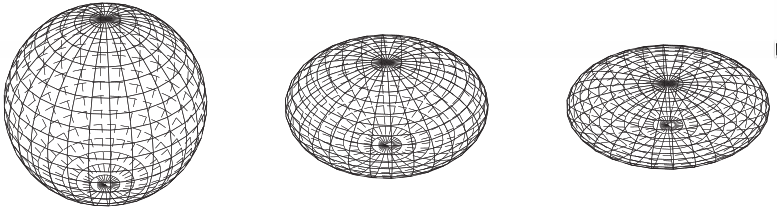
\includegraphics[width=\textwidth]{figures/topology_sphere.png}
        \caption{Topological 2-spheres}
    \end{center}
\end{figure}

All these shapes have the same topology but, since
the distance between the points on the surface has changed, they have different
geometries.

\subsection{Some Basic Set Terminologies}
\textbf{a. Open and Closed Sets:} A subset S of X is said to be an \textbf{open set} if every point of S is an interior point of S i.e. \\
$\forall$ x $\epsilon$ S $\exists \: \epsilon >$ 0 s.t. B(x; $\epsilon$) $\subset$ S.

A subset S of X is called a \textbf{closed set} if $\overline{\text{S}}$ = X-S is open.

Some sets may be both open and closed, such sets are called \textbf{clopen sets}.

\textbf{b. Interior and Exterior: } Let S $\subset \mathbb{R}$ and x $\epsilon$ S then x is said to be an \textbf{interior point} of S if 
$\exists$ B(x; r) s.t. B(x; r) $\subset$ S. The set of all interior points of S is called the \textbf{interior} of S, \textbf{int(S)}.
Consequently, the union of all open sets contained in S is the int(S).

Similarly, x is called an \textbf{exterior point} of S if x is an interior point of X-S and the set of all exterior points of S
is called the \textbf{exterior} of S, \textbf{ext(S)}.

\textbf{c. Closure: } Closure of S $\subset$ X, \textbf{Cl(S)} is the intersections of all the closed sets cotaining S.
Set S is called \textbf{dense} if Cl(S) = X.

\textbf{d. Cover: } An \href{https://en.wikipedia.org/wiki/Cover_(topology)}{\textbf{open cover}} of S $\subset$ X is a collection of {U$_\alpha$} of open sets in X
whose union contains S i.e.\\
S $\subseteq$ U$_\alpha$

An open cover is \textbf{locally finite} if, for every x $\epsilon$ S , there is an open neighborhood B(x; r) of x
such that $\lvert$\{$\alpha$: U $\cap$ U$_\alpha$ $\neq \: \emptyset $\}$\rvert$ is finite. (Note that a locally finite open cover is not
necessarily finite.) An open cover {V$_\beta$ } is a \textbf{refinement} of {U$_\alpha$} if for all $\beta$ there is
an $\alpha$ such that U$_\alpha \supset$ V$_\beta$ .

\textbf{e. Compact: } A topological space X is \href{https://blogs.scientificamerican.com/roots-of-unity/what-does-compactness-really-mean/}{\textbf{compact}}
if every open cover has a finite subcollection that also covers X (“every open cover has a finite \textbf{subcover}”). 
Intuitively, compact spaces can be thought of as being finite in extent. 
For example, a subset of Euclidean space is compact if and only if it is closed and
bounded (\href{https://en.wikipedia.org/wiki/Heine%E2%80%93Borel_theorem}{\textbf{Heine-Borel theorem}}).

A \textbf{base/basis} for a topology $\tau$ of a topological space (X, $\tau$) is a family/collection, $\mathcal{B}$ of 
open sets of X s.t. every open set of the topology is equal to the union of some sub-family of $\mathcal{B}$ ($\mathcal{B}$ spans $\tau$).
Eg: the set of all open intervals in real number line $\mathbb{R}$ is a basis for Euclidean topology on $\mathbb{R}$ because every open
interval is an open set, and every open subset of $\mathbb{R}$ can be written as a union of some family of open intervals. The topology generated by $\mathcal{B}$ is just the collection of  open subsets of X where U is considered open
if $\forall$ x $\epsilon$ U $\exists$ B $\epsilon \: \mathcal{B}$ s.t. x $\epsilon$ B $\subset$ U.

Given two sets X and Y , the \textbf{product topology} on X $\times$ Y is the topology generated
by all sets of the form U $\times$ V, where U is open in X and V is open in Y. 
For Eg: The standard topology on $\mathbb{R}^n$ is the product topology on $\underbrace{\mathbb{R} \times ... \times \mathbb{R}}_{n \:times}$.

\subsection{Mapping Between Topologies}
Let f: X $\rightarrow$ Y be a map between topological spaces. The map f is \textbf{continuous}
if the inverse image of an open set S in Y is open in X.

Let $\tau$ be a topology on X, and let Y $\subset$ X. 
The collection $\tau_Y$ = {Y $\cap$ U: U $\epsilon \: \tau$} is a topology on Y, called the \textbf{induced topology} or \textbf{subspace topology} on Y. 
The space Y equipped with this topology is a \textbf{subspace} of X.

A map f: X $\rightarrow$ Y between topological spaces is a \textbf{homeomorphism} if it is
continuous with continuous inverse, meaning that there is a continuous map g: Y $\rightarrow$ X  such that g $\circ$ f = f $\circ$ g = 1. 
If such a pair of maps exist, we write X $\approx$ Y and say that X and Y are \textbf{homeomorphic} (or \textbf{topologically equivalent}). 
A \textbf{property} P(X) is a \textbf{topological invariant} of X if X $\approx$ Y implies P(X) = P(Y) i.e.
P(X) depends only on the topology of X. The property P(X) is a \textbf{complete topological invariant} of a space X provided that P(X) = P(Y) iff X $\approx$ Y. 
Topology can be loosely characterized as the study of the topological invariants of spaces.

\subsection{Multivariable Calculus} \label{Multivariable Calculus}
Let U $\subset \mathbb{R}^n$ be an open set and suppose that f: U $\rightarrow \mathbb{R}$ is a function. 
Label the points of $\mathbb{R}^n$ by the n-tuples x = (x$^1$, ..., x$^n$ ). Then the \href{https://en.wikipedia.org/wiki/Partial_derivative}{partial derivative} $\partial$f /$\partial$x$^i$
is defined by
\begin{equation}
    \frac{\partial f}{\partial x^i} = \lim_{h \rightarrow 0} \frac{f(x+he_i) - f(x)}{h}
\end{equation}

where e$_i$ = (0, ..., 1, ..., 0) has a “1” in the ith slot. For higher order, let $\alpha$ = (i$_1$, ..., i$_k$). Then
\begin{equation}
    \frac{\partial f}{\partial x^\alpha} (x) = \frac{\partial^k f}{\partial x^{i_1} ... \partial x^{i_k}}
\end{equation}

A function f: $\mathbb{R}^n$ $\rightarrow \mathbb{R}$ is \textbf{C$_\infty$}, or \href{https://en.wikipedia.org/wiki/Smoothness}{\textbf{smooth}}, 
if $\frac{\partial f}{\partial x^\alpha}$ exists and is continuous for
all $\alpha$. The composition of smooth functions is smooth.

Let U $\subset \mathbb{R}^n$ be an open set but now suppose that f: U $\rightarrow \mathbb{R}^m$ is a map,
given by x $\rightarrow$ (f$^1$(x), ..., f$^m$(x)). The map f is smooth if each component
function f$^1$ is smooth. The derivative D f(x) of f at x is just the matrix of partial
derivatives D f(x) = ($\partial f^i / \partial x^j$); this matrix is called the \href{https://en.wikipedia.org/wiki/Jacobian_matrix_and_determinant}{\textbf{Jacobian matrix}}.
When n = m, its determinant det($\partial f^i / \partial x^j$) is called the Jacobian determinant or more
simply the \textbf{Jacobian} of the map f.

Let U, V $\subset \mathbb{R}^n$ be two open sets, and let f: U $\rightarrow$ V be a homeomorphism.
If f and f$^{-1}$ are both smooth then f is called a \href{https://en.wikipedia.org/wiki/Diffeomorphism}{\textbf{diffeomorphism}} (isomorphism of smooth manifolds).
Since every diffeomorphism is a homeomorphism, given a pair of manifolds which are diffeomorphic to each other they are in particular homeomorphic to each other. 
The converse is not true in general. This brings us to the all-important \textbf{inverse function theorem (IFT)} which states, "if the matrix
representing the derivative of a function is invertible at some point then the function
itself is a \href{https://en.wikipedia.org/wiki/Local_diffeomorphism}{local diffeomorphism} in the neighborhood of that point".

\subsection{Coordinate Systems}
\href{https://en.wikipedia.org/wiki/N-sphere}{2-sphere}

Consider the transformation in $\mathbb{R}^2$ between Cartesian and polar coordinates:
\begin{equation}
    \begin{aligned}
        x = r cos\theta \\
        y = r sin \theta
    \end{aligned}
\end{equation}

Every point in the plane can be described uniquely in the (x, y) coordinate system,
but the \textbf{origin} is a problem for the polar coordinate system because it is described
by the infinity of pairs (r, $\theta$) = (0, anything). Another way to see that something
strange happens at the origin is to compute the Jacobian of the transformation.
\begin{equation}
    \begin{vmatrix}
        \partial x / \partial r & \partial x / \partial \theta \\ 
        \partial y / \partial r & \partial y / \partial \theta 
   \end{vmatrix} = 
   \begin{vmatrix}
    cos \theta & -r sin \theta \\ 
    sin \theta & r cos \theta 
\end{vmatrix} = r
\end{equation}

Now, at origin r vanishes and consistently the Jacobian determinant.

The \textbf{IFT} provides the link between these two ways of
determining the validity of a given coordinate transformation. A coordinate transformation is a good one 
if there is a one-to-one correspondence between the two sets of coordinates and if the transformation is differentiable.
In other words, a set of functions {f$^i$(x)} on $\mathbb{R}^n$ constitutes a \textbf{good coordinate system} in the 
neighborhood of a point x if the transformation (x$^1$, ..., x$^n$ ) $\rightarrow$ (f$^1$ (x$^1$, ..., x$^n$ ), ..., f$^n$ (x$^1$, ..., x$^n$)) is a diffeomorphism.
Ascertaining whether a map is a diffeomorphism can be difficult. 
But checking whether a Jacobian vanishes is usually easy. 
The \textbf{IFT} assures that, as long as the Jacobian of the transformation is nonsingular, 
we can coordinatize the neighborhood of x with the functions f$^i$.

\subsection{Differential Manifold (Smooth Manifold or C\texorpdfstring{$_\infty$ } d)}
An n-dimensional smooth manifold \textbf{M} consists of a  \href{https://en.wikipedia.org/wiki/Hausdorff_space}{\textbf{Hausdorff} topological space}
together with a \textbf{countable} collection of open sets \{U$_i$\}, called \textbf{coordinate neighborhoods/patches}, 
that \textbf{cover} \textbf{M} and a collection of maps \{$\psi_i$\}, called \textbf{coordinate
maps}, satisfying two conditions.

1. Each $\psi_i$: U $\rightarrow \mathbb{R}^n$ is a homeomorphism onto an open subset of Rn . (We say
that \textbf{M} is \textbf{locally Euclidean}.) \\
2. If U$_i$ and U$_j$ are two overlapping coordinate neighborhoods with coordinate maps $\psi_i$ and $\psi_j$ 
then $\psi_j \circ$ $\psi_i^{-1}$: $\psi_i$ (U$_i$ $\cap$ U$_j$) $\rightarrow \psi_j$ (U$_i$ $\cap$ U$_j$) is
a diffeomorphism. (We say that the coordinate maps are \textbf{compatible} on
overlaps.)

Each pair (U$_i$ , $\psi_i$) is called a \textbf{coordinate chart}, and the collection of all coordinate
charts is called an \textbf{atlas}. The maps $\psi_j \circ$  $\psi_i^{-1}$ are called \textbf{transition functions} of the
atlas.

The \href{https://www.quora.com/What-is-the-significance-of-Hausdorff-Spaces-How-do-these-measurements-help-us-What-does-it-allow-us-to-have}{\textbf{Hausdorff condition}}
is there basically to express our intuition of space as “infinitely divisible”, so that we can separate points with open sets. 
The condition that the \textbf{cover be countable} is there for a technical reason having to do
with extending locally defined quantities to globally defined ones. 
The condition that \textbf{M} be \textbf{locally Euclidean} serves at least two purposes. 
First, it tells us that, in the neighborhood of a point, all n-dimensional manifolds look like a (mildly deformed) bit of Euclidean n-space. 
Second, it allows us to define local coordinates so that we can compute things. 
The compatibility condition ensures that we can patch together the coordinate systems consistently, so that we always end up with valid coordinates.
\begin{figure}
    \begin{center}
        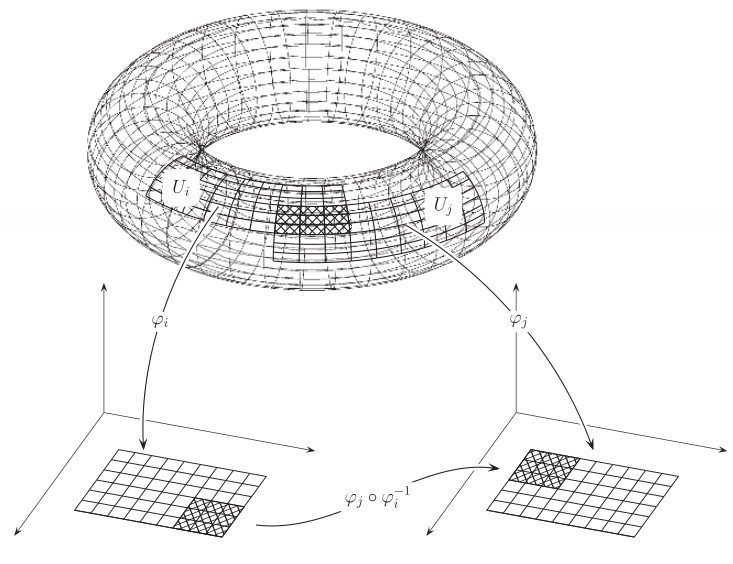
\includegraphics[width=0.75\textwidth]{figures/coordinate-chart.png}
        \caption{Two coordinate charts and a transition function}
    \end{center}
\end{figure}

Let (U, $\psi$) be a coordinate chart with p $\epsilon$ U and suppose that $\psi$(p) = q. If
x$^1$ , . . . , x$^n$ are the standard coordinate functions on $\mathbb{R}^n$ then q has coordinates
(x$^1$(q), . . . , x$^n$(q)). Thus we can write
\begin{equation}
    \psi(p) = (x^1(q), . . . , x^n(q))
\end{equation}

The functions x$^1$ , . . . , x$^n$, viewed as functions on U , are called \textbf{local coordinates} on U. 
Let V be another coordinate neighborhood, with local coordinates y$^1$ , . . . , y$^n$. 
If U$\cap$V = $\phi$ then on $\psi$(U$\cap$V) the action of the transition function $\psi_1 \circ$  $\psi_2^{-1}$ can be
written in local coordinates as follows:
\begin{equation}
    (x^1 , . . . , x^n ) \rightarrow (y^1 (x^1 , . . . , x^n ), . . . , y^n (x^1 , . . . , x^n ))
    \label{eqn:local_coord}
\end{equation}

The compatibility condition (2) in the definition of a manifold is just the statement that equation \ref{eqn:local_coord} is a diffeomorphism, which, by the inverse
function theorem, is equivalent to the requirement that the Jacobian determinant
det($\partial$y$_i$/$\partial$x$_j$) be nonzero. The sign of this determinant is important. 
A manifold is said to be \href{https://en.wikipedia.org/wiki/Orientability}{\textbf{orientable}}
if it is possible to choose an ordering of the local coordinates so that the Jacobian
determinants of the transition functions have the same sign on every pair of overlapping neighborhoods. 
If this is possible then the manifold has two opposite orientations, according to the choice of sign.

\subsection{Smooth Maps on Manifolds}
The definition of the derivative given in Section \ref{Multivariable Calculus} uses the linear structure of
Euclidean space in a crucial way, and there is no way to define something similar
for a general curved space. Instead, the existence of the coordinate maps on
a smooth manifold is used to define differentiability.

A function f: \textbf{M} $\rightarrow \mathbb{R}$ is smooth at p $\epsilon$ \textbf{M} if, for any chart (U, $\psi$)
with p $\epsilon$ U, the map
\begin{equation}
    \widetilde{f}= f \circ \psi^{-1}:\psi(U) \rightarrow \mathbb{R}
\end{equation}

is a smooth function in the usual Euclidean sense near $\psi$(p).

In general, Let \textbf{M} and \textbf{N} be two smooth manifolds of dimensions m and n, respectively. 
A map f: \textbf{M} $\rightarrow$ \textbf{N} is smooth if $\forall$ p $\epsilon$ \textbf{M} $\exists$ charts (U, $\psi_1$) on \textbf{M} and (V, $\psi_2$) on \textbf{N}, 
with p $\epsilon$ U and f(U) $\subset$ V s.t.
\begin{equation}
    \widetilde{f}= \psi_2 \circ f \circ \psi_1^{-1}:\psi_1(U) \rightarrow \psi_2(V)
\end{equation}

is a smooth map of Euclidean spaces. A smooth map f: \textbf{M} $\rightarrow$ \textbf{N} is a \textbf{diffeomorphism} 
if f$^{-1}$ exists and is smooth, in which case we say that \textbf{M} and \textbf{N} are diffeomorphic.

Because smooth maps of manifolds reduce to smooth maps of Euclidean space, 
the inverse function theorem works for manifolds in the same way as it does in Euclidean space: 
if the Jacobian matrix of f is nonsingular then f is a local diffeomorphism. 
In particular, M and N can only be \textbf{diffeomorphic} if m = n.

\subsection{\href{https://mathweb.ucsd.edu/~eizadi/250A-2019/Patrick-Girardet.pdf}{Immersion and Embedding}}
A prototypical theme in geometry is the study of “\textbf{spaces with structure}”, i.e.
a set X equipped with some sort of additional geometric structure, such as a
topology in the case of topological spaces. It is important how
functions between our spaces with structure interact with the structure on those
spaces. We concern ourselves only with those functions which “preserve” the
structure (e.g. \textbf{differentiable maps} between {differentiable manifolds}, 
which are maps respecting the differentiable structure).

A differentiable mapping f: \textbf{M}$^m \rightarrow$ \textbf{N}$^n$ (m = dim \textbf{M}, n = dim \textbf{N})
of differentiable manifolds \textbf{M} and \textbf{N} is said to be an \href{https://en.wikipedia.org/wiki/Immersion_(mathematics)}{immersion}
if df$_p$: T$_p$\textbf{M} $\rightarrow$ T$_{f(p)}$\textbf{N} is injective $\forall$ p $\epsilon$ \textbf{M} where
T$_p$\textbf{X} denotes the \textbf{tangent space} [\ref{Tangent Space}] of manifold \textbf{X} at point p $\epsilon$ \textbf{X}.

Equivalently, f is an immersion if its derivative \textbf{df} has a constant rank = m i.e. rank(df) = dim \textbf{M} = m.
The function itself need not be injective, only its derivative \textbf{df} must be.

Since df: T$_p$\textbf{M} $\rightarrow$ T$_{f(p)}$\textbf{N} is a linear map between vector spaces
and dim T$_p$\textbf{M} = dim \textbf{M} = m $\forall$ p $\epsilon$ \textbf{M}, 
it follows by linear algebra that if df is an immersion then dim \textbf{M} $\leq$ dim \textbf{N}. 
We call dim \textbf{N} - dim \textbf{M} the \textbf{codimension} of df.
\begin{figure}[h]
    \begin{center}
        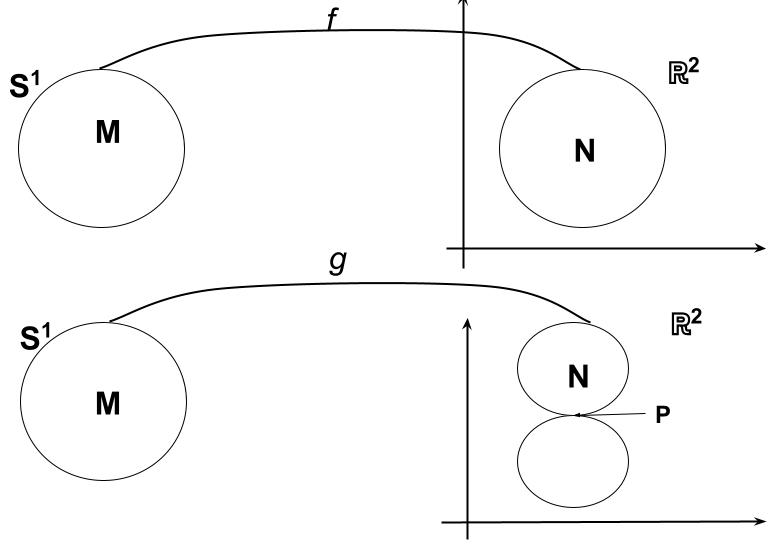
\includegraphics[width=0.5\textwidth]{figures/embedding-immersion.png}
        \caption{\textit{f} is an immersion as well as embedding but \textit{g} is only immersion due to self-intersection at p, which doesn't allow homeomorphism.}
    \end{center}
\end{figure}

If f is an immersion $\forall$ p $\epsilon$ \textbf{M} then \textbf{M} is an (immersed) \textbf{submanifold} of \textbf{N}.
The Jacobian has \textbf{maximal rank} (namely m), so f(M) is locally coordinatizable according to the IFT. 
If m $\geq$ n and the Jacobian of the transformation has maximal rank (namely n) at p $\epsilon$ \textbf{M} then f is called a
\textbf{submersion} at p.

An injective immersion f is called an \textbf{embedding} provided
that f maps \textbf{M} homeomorphically onto its image f(\textbf{M}) (in the induced topology). 
The basic difference between immersions and embeddings is that the image
of an immersion can have \href{https://en.wikipedia.org/wiki/List_of_self-intersecting_polygons}{\textbf{self-intersections}} 
whereas the image of an embedding cannot. 

The \href{https://en.wikipedia.org/wiki/Whitney_embedding_theorem}{\textbf{Whitney embedding theorem}} says that
any n-dimensional topological manifold can be embedded in $\mathbb{R}^{2n+1}$, and any n-dimensional smooth manifold can be embedded in $\mathbb{R}^{2n}$.
The  Möbius strip is a smooth 1-manifold and can be embedded in $\mathbb{R}^{3}$ and 
the Klein bottle is a smooth 2-manifold and thus can be embedded in $\mathbb{R}^{4}$. 
If you try to construct the Klein bottle in $\mathbb{R}^{3}$, 
you will observe that you cannot do it without creating self-intersections somewhere.
Whitney's result means that, without loss of generality, we could simply treat
manifolds as living in a large Euclidean space. The intrinsic description of a manifold also has physical utility. Einstein modeled
the universe as a smooth manifold of a certain type.

\begin{figure}[h]
    \begin{center}
        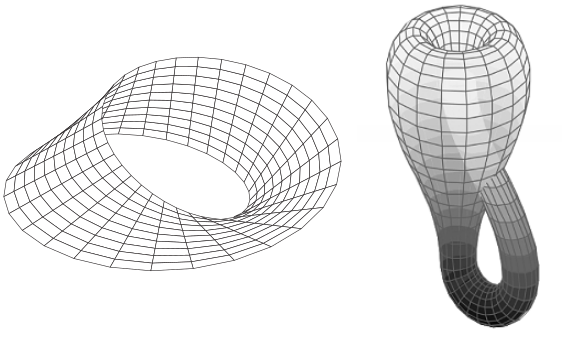
\includegraphics[width=0.5\textwidth]{figures/moebius-klien.png}
        \caption{Möbius strip immersed in $\mathbb{R}^{2}$ (left) and Klein bottle immersed in $\mathbb{R}^{3}$ (right)}
    \end{center}
\end{figure}

\subsection{Tangent Space}\label{Tangent Space}
The \href{https://en.wikipedia.org/wiki/Tangent_space}{\textbf{tangent space}} is a space spanned by
the tangent vectors of curves lying in that space. The tangent space of a manifold generalizes to higher dimensions 
the notion of tangent planes to surfaces in 3D and tangent lines to curves in 2D. 
In the context of physics the tangent space to a manifold at a point can be viewed as the space of possible velocities 
for a particle moving on the manifold ($\overrightarrow{v}$ = $\partial \overrightarrow{r}/ \partial t$).

Once the tangent spaces of a manifold have been introduced, one can define vector fields, which are abstractions of the velocity field of particles moving in space. 
A vector field attaches to every point of the manifold a vector from the tangent space at that point, in a smooth manner. 
Such a vector field serves to define a generalized ordinary differential equation on a manifold: 
A solution to such a differential equation is a differentiable curve on the manifold whose derivative at any point is equal to the 
tangent vector attached to that point by the vector field. 
All the tangent spaces of a manifold can be glued together to form a new differentiable manifold
with twice the dimension of the original manifold, called the \href{https://en.wikipedia.org/wiki/Tangent_bundle}{\textbf{tangent bundle}}
of the manifold.

Let us define a tangent vector X$_p$ at a point p $\epsilon$ \textbf{M} to be a \textbf{linear derivation} at p. 
This means that, $\forall$ a, b $\epsilon$ $\mathbb{F}$ and
f, g $\epsilon$ $\Omega^0$(\textbf{M}), X$_p$ : $\Omega^0$(\textbf{M}) $\rightarrow \mathbb{R}$ satisfies

1. \textbf{linearity}: X$_p$ (af + bg) = a X$_p$ (f) + bX$_p$ (g), and \\
2. \textbf{Leibniz property}: X$_p$ (f g) = g(p)X$_p$ (f) + f (p)X$_p$ (g).

The vector space T$_p$\textbf{M} generated by all the X$_p$ is called the \textbf{tangent space to
M at p}. It is important to note that the tangent space T$_p$\textbf{M} is defined independently of any
coordinate system. Thus, at each point we are free to pick any basis \{e$_i$\}, not just
a coordinate basis \{$\partial$/$\partial$ x$_i$\}. Any smoothly varying basis on \textbf{M} is called a \textbf{frame field}.
Generally, frame fields do not exist everywhere on \textbf{M}; they clearly exist
locally, because e$_i$ = $\partial$/$\partial$ x$_i$  is an instance. In terms of a frame field \{e$_i$\}, we could
write a vector field X as
\begin{equation}
    X = X_i e_i
\end{equation}

\begin{figure}[h]
    \begin{center}
        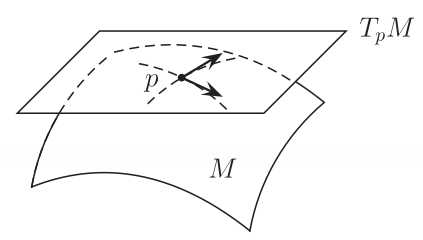
\includegraphics[width=0.5\textwidth]{figures/tangent-space.png}
        \caption{Although the tangent space T$_p$\textbf{M} is an abstract linear space attached to
        \textbf{M} at p, we often imagine it to look like above figure.}
    \end{center}
\end{figure}

\subsection{Cotangent Space}
The cotangent space $T_{p}^{*}$\textbf{M} is defined as the dual space of the tangent space at p, 
$T_{p}$\textbf{M}. The elements of the cotangent space are called \textbf{cotangent vectors} or \textbf{tangent covectors}.
All cotangent spaces at points on a connected manifold have the same dimension, equal to the dimension of the manifold. 
All the cotangent spaces of a manifold can be "glued together" (i.e. unioned and endowed with a topology) to form a new differentiable manifold of twice the dimension, the cotangent bundle of the manifold.

Let  \textbf{M} be a smooth manifold and let  p be a point in \textbf{M}. 
Let  $T_{p}$\textbf{M} be the tangent space at p. 
Then the cotangent space at p is defined as the dual space of $T_{p}$\textbf{M}:
\begin{equation}
    T_{p}^{*}\textbf{M} = (T_{p}\textbf{M})^{*}
\end{equation}
Concretely, elements of the cotangent space are \textbf{linear functionals} on 
$T_{p}$\textbf{M} i.e. every element $\alpha \: \epsilon \: T_p$\textbf{M} is a linear map
$\alpha$ :$T_{p}$\textbf{M} $\rightarrow \mathbb{F}$

where $\mathbb{F}$ is the underlying field of the vector space being considered, for example, the field of real numbers. 
The elements of $T_{p}^{*}$\textbf{M} are called cotangent vectors.

Let \{x$^i$\} be local coordinates  around p, then T$_p$\textbf{M} is spanned by the n basis vectors $\partial/\partial x^i$. The
corresponding dual basis vectors are denoted dx$^i$. By definition we have
\begin{equation}
    \Bigg< \frac{\partial}{\partial x_i}, dx^j\Bigg> = \delta_i^j
\end{equation}

A general element $\alpha$ p of T$_p^*$\textbf{M} is a linear combination of
the basis elements:
\begin{equation}
    \alpha_p = a_i dx^i
\end{equation}
where $\alpha_i$ are constants.

A \textbf{differential} \href{https://mathworld.wolfram.com/One-Form.html}{\textbf{1-form}} or \textbf{smooth covector field}
on \textbf{M} is a smooth map p$\rightarrow \alpha_p$. In local coordinates around p 
\begin{equation}
    \alpha = a_i(x)dx^i
\end{equation}
where the a$_i$(x) are smooth functions on \textbf{M}.

\textbf{1-forms} (covector/pseudovector) of a vector space with local coordinates (dx$_1$, dx$_2$, ..., dx$_n$)
are the elements of a vector space with local basis (dx$^1$, dx$^2$, ..., dx$^n$) i.e. dual space.
(Vectors (covariant vectors/\textbf{kets} $|\psi \rangle$) and 1-forms (contravariant vectors/\textbf{bras} $\langle \psi |$) are dual to each other.)
\textbf{2-forms} are the elements of the exterior product space with local basis (dx$^1 \exterior$ dx$^2$, dx$^2 \exterior$ dx$^3$ ..., dx$^{n-1} \exterior$ dx$^n$).
In general, (\href{https://www.physicsforums.com/threads/what-is-2-form.762846/#:~:text=The%201%2Dforms%20(or%20covectors,the%20bases%20may%20be%20omitted.}{\textbf{p-form}})
are the elements of the exterior product space with basis (dx$^1 \exterior$ dx$^2 ... dx^p$, ...). For eg:
in 3D Euclidean space with basis (i, j, k), 

1-form have basis (i', j', k') \\
2-form have basis (j$\exterior$k, k$\exterior$i, i$\exterior$j) \\
3-form have basis (i$\exterior$j$\exterior$k) \\
other higher forms don't exist for 3D.

Like tangent space, cotangent space is also independent of any particular coordinate system for its definition. 
If \{e$_i$\} is a generic basis for T$_p$\textbf{M} then the corresponding dual basis \{$\theta^i$\} is called a \textbf{coframe field}, so
\begin{equation}
    \Big<e_i, \theta^j\Big> = \delta_i^j
\end{equation}

\subsection{Cotangent Space as \href{https://en.wikipedia.org/wiki/Jet_(mathematics)}{Jet Space} }
We have defined a differential 1-form as a smoothly varying map
on M that assigns to every point p of M an element of the cotangent space at p.
Although this is correct, it is perhaps rather unsatisfying because the cotangent
space is defined in terms of the tangent space, which is itself defined as a space of
derivations on functions. There is, however, an elegant way to define the cotangent
space directly, using just the notion of a smooth function, which is perhaps a bit
more natural from the point of view of manifold theory. It uses the idea of a \textbf{jet}.
Jet is an operation that takes a differential function \textit{f} and produces a polynomial,
the truncated Taylor polynomial of \textit{f} at each point of its domain. 
The theory of jets regards these polynomials as abstract polynomials rather than polynomial functions.
\begin{equation}
    (J_{x_0}^k f)(z) = \sum_{i=0}^{k} \frac{f^{(i)}(x_0)}{i!}z^i = f(x_0) + f'(x_0)z + ... + \frac{f^{(k)}(x_0)}{k!}z^k
\end{equation}
gives the k-jet of f:$\mathbb{R} \rightarrow \mathbb{R}$ at point x$_0$ in 1D case.

Let C$^\infty$($\mathbb{R}^n, \mathbb{R}^m$) be a vector space of smooth functions f:$\mathbb{R}^n \rightarrow \mathbb{R}^m$.
Let k is a non-negative integer and p $\epsilon \mathbb{R}^n$, then we can define an equivalence relation \textbf{E}$^k_p$ on C$^\infty$
by declaring that two functions \textit{f} and \textit{g} are equivalent to the order of k if they have the same value at p,
and all their partial derivatives agree at p upto their kth derivatives i.e.
\textit{f} $\sim$ \textit{g} iff \textit{f}-\textit{g} = 0 to kth order.
The \textbf{kth order jet space} of C$^\infty$($\mathbb{R}^n, \mathbb{R}^m$) at p is defined as the set of 
equivalence classes of \textbf{E}$^k_p$ and is denoted by J$^k_p$($\mathbb{R}^n, \mathbb{R}^m$).

Now, let \textit{f}:\textbf{M} $\rightarrow \mathbb{R}$ be a smooth function, p$\epsilon$\textbf{M}, and \{x$^i$\} local coordinates around
p. We say that \textit{f} vanishes to first order at p if $\partial f /\partial x^i$ vanishes at p for all i.
for k$\geq$1 we say that \textit{f} vanishes to kth order at p if, $\forall$ i, $\partial f /\partial x^i$ vanishes to (k-1)th order at p,
where \textit{f} vanishes to zeroth order at p if \textit{f}(p) = 0. 
In other words, \textit{f} vanishes to kth order at p if the first k terms in its Taylor expansion vanish at p.

For k$>$0 let \textbf{M}$^k_p$ be the set of all smooth functions on \textbf{M} vanishing to (k-1)th order at p, 
and set \textbf{M}$^0_p$:= $\Omega^0$(\textbf{M}) and M$_p$ := \textbf{M}$^1_p$. Each \textbf{M}$^k_p$ is a vector
space under the usual pointwise operations, and we have the series of inclusions

\textbf{M}$^0_p \supset$ \textbf{M}$^1_p \supset$ \textbf{M}$^2_p \supset$ ....

We now define T$_p^*$\textbf{M}, the cotangent space to \textbf{M} at p, to be the
\href{https://www.youtube.com/watch?v=nh-YgZph-r4}{\textbf{quotient space}} 
\begin{equation}
    T_p^*\textbf{M} = \textbf{M}_p/\textbf{M}^2_p
\end{equation}
An element of T$_p^*$\textbf{M} is called a \textbf{differential 1-form} at p.
\newpage

\section{GROUP THEORY}
\subsection{Group Definition}
A \textbf{Group} G, is a set with a rule for assigning to every (ordered) pair of
elements, a third element, satisfying:

1. If f, g $\epsilon$ G then h = fg $\epsilon$ G. \\
2. Associativity: $\forall$ f, g, h $\epsilon$ G, f(gh) = (fg)h. \\
3. Existence of identity element: $\forall$ f $\epsilon$ G $\exists$ \textit{e} s.t. \textit{e}f = f\textit{e} = f. \\
4. Existence of inverse element: $\forall$ f $\epsilon$ G $\exists$ f $^{-1}$ s.t. f f$^{-1}$ = f$^{-1}$f = \textit{e}.
\begin{figure}[h]
    \centering
    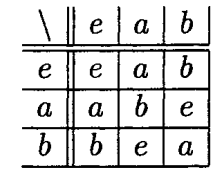
\includegraphics[width=0.3\textwidth]{figures/z3-group.png}
    \caption{Z$_3$ group multiplication table. (Every row and column
    of the multiplication table contains each element of the group exactly once.
    This must be the case because the inverse exists.)}
\end{figure}

A group G is \textbf{finite} if it has a finite number of elements. Otherwise it is \textbf{infinite}.
The number of elements in a finite group G is called the \textbf{order} of G. For eg: Z$_3$, the cyclic group of order 3.

An \textbf{Abelian group} G in one in which the multiplication law is commutative i.e.
g$_1$g$_2$ = g$_2$g$_1$. And the one which doesn't follows commutation is called \textbf{non-Abelian group}.

\subsection{Representation}
A \textbf{Representation} of a group G is a mapping D of the elements of G onto a set of
linear operators with the following properties:

1. D(\textit{e}) = 1, where 1 is the identity operator in the space on which
the linear operators act. \\
2. D(g$_1$)D(g$_2$) = D(g$_1$g$_2$) i.e. the group multiplication law 
is mapped onto the natural multiplication in the linear space on which the linear operators act.

For eg: representation of Z$_3$ is,
\begin{equation}
    D(e) = 1, \hspace{1cm} D(a) = e^{2\pi i/3}, \hspace{1cm} D(b) = e^{4\pi i/3}
\end{equation}
another representation of Z$_3$ can be directly constructed from the multiplication table as,
\begin{equation}
    D(e) = \begin{pmatrix}
        1 & 0 & 0 \\ 
        0 & 1 & 0 \\ 
        0 & 0 & 1 \\ 
   \end{pmatrix}, \hspace{1cm} 
   D(a) = \begin{pmatrix}
        0 & 0 & 1 \\ 
        1 & 0 & 0 \\ 
        0 & 1 & 0 \\ 
   \end{pmatrix}, \hspace{1cm} 
   D(b) = \begin{pmatrix}
        0 & 1 & 0 \\ 
        0 & 1 & 1 \\ 
        1 & 0 & 0 \\ 
\end{pmatrix},
\end{equation}

By taking the group elements themselves to form an orthonormal basis for a vector space, 
$|e \rangle$, $|a\rangle$, and $|b\rangle$ we can also define \textbf{regular representation} as,
\begin{equation}
    D(g_1)|g_2\rangle = |g_1g_2\rangle
    \label{eqn:representation}
\end{equation}

The \textbf{dimension of a representation} is the dimension of the space on which
it acts and the dimension of the regular representation is the order of the group. The representation of Z$_3$ is 1 dimensional.
For any finite group, we can define a vector space in which the basis vectors are labeled by the group elements.
Then equation \ref{eqn:representation} defines the regular representation.

\subsection{Subgroup}
A group H whose elements are all elements of a group G is called a subgroup of G. 
The identity, and the group G are trivial subgroups of G. For eg., the permutation group S3, has a Z3 subgroup formed by the elements \{e, a$_1$, a$_2$\}. 
Subgroup can be used to divide up the elements of the group into subsets called \href{https://en.wikipedia.org/wiki/Coset}{\textbf{cosets}}.
Given an element \textit{g} of G, the \textbf{left cosets} of H in G are the sets obtained by multiplying each element of H by a fixed element \textit{g} of G (where \textit{g} is the \textbf{left factor})
\begin{center}
    \textit{g}H = \{\textit{g}h : h $\epsilon$ H\} $\forall$ \textit{g} $\epsilon$ G.
\end{center}
The \textbf{right cosets} can be defined similarly where g is now a \textbf{right factor}.
\begin{center}
    H\textit{g} = \{h\textit{g} : h $\epsilon$ H\} $\forall$ \textit{g} $\epsilon$ G.
\end{center}

The number of elements in each coset is the order of H. Every element of G
must belong to one and only one coset. Thus for finite groups, the order of
a subgroup H must be a factor of order of G. 
A subgroup H of G is called an \textbf{invariant} or \textbf{normal subgroup} if $\forall$ g$\epsilon$G
\begin{equation}
    gH = Hg
\end{equation}

i.e.$\forall$ \textit{g} $\epsilon$G and \textit{h}$_1 \: \epsilon$ H $\exists$ an \textit{h}$_2 \: \epsilon$ H s.t.
\begin{center}
    \textit{h}$_1$\textit{g} = \textit{gh}$_2$, or \textit{gh}$_2$\textit{g}$^{-1}$ = \textit{h}$_2$.
\end{center} 

The trivial subgroups e and G are invariant for any group. If H is invariant then H\textit{g}$_1$ H\textit{g}$_1^{-1}$ = H, 
so the product of elements in two cosets is in the coset represented by the product of the elements. 
In this case, the coset space G/H, is called the \textbf{factor group} of G by H.

The \textbf{center} of a group G is the set of all elements of G that commute
with all elements of G. The center is always an Abelian, invariant subgroup
of G. However, it may be trivial, consisting only of the identity, or of the
whole group.

The \textbf{characters} $\chi_D$(g) of a group representation D are the traces of the linear
operators of the representation or their matrix elements:
\begin{equation}
    \chi_D(g) \equiv Tr D(g) = \sum_{i}[D(g)]_{ii}
\end{equation}

The advantage of the characters is that because of the cyclic property of the trace Tr(AB) = Tr(BA), they are unchanged by similarity transformations,
thus all equivalent representations have the same characters. The characters are also different for each inequivalent irreducible representation, D$_a$\textemdash 
in fact, they are orthonormal up to an overall factor of N.

\subsection{Eigenstates}
In quantum mechanics, we are often interested in the eigenstates of an invariant hermitian operator, in particular the Hamiltonian, H. 
We can always take these eigenstates to transform according to irreducible representations of the symmetry group. 
To prove this, note that we can divide up the Hilbert space into subspaces with different eigenvalues of H. 
Each subspace furnishes a representation of the symmetry group because D(\textit{g}), the group representation on the full Hilbert space, 
cannot change the H eigenvalue because [D(\textit{g}), H] = 0. But then we can completely reduce the representation in each subspace.
If some irreducible representation appears only once in the Hilbert space, then the states in that representation must be eigenstates
of H (and any other invariant operator). This is true because H$|a, j, x\rangle$ must be in the same irreducible representation, thus
\begin{equation}
    H|a, j, x\rangle = \sum_{y} c_y |a, j, x\rangle
\end{equation}
and if x andy take only one value, then $|a, j, x\rangle$ is an eigenstate.

\textbf{Theorem:} If a hermitian operator H, commutes with all the elements D(\textit{g}), of a representation of the group G, 
then you can choose the eigenstates of H to transform according to irreducible representations of G. 
If an irreducible representation appears only once in the Hilbert space, every state in the irreducible representation 
is an eigenstate of H with the same eigenvalue.

For Abelian groups, this procedure of choosing the H eigenstates to transform under irreducible representations is analogous to simultaneously 
diagonalizing H and D(\textit{g}) because for an Abelian group that commutes with the H, the group elements can simultaneously
diagonalized along with H. This is a consequence of theorem,

\textbf{Theorem:} All of the irreducible representations of a finite Abelian group are 1-dimensional.

For a non-Abelian group, we cannot simultaneously diagonalize all of the D(\textit{g})s, 
but we can completely reduce the representation on each subspace of constant H.
A classical problem which is quite analogous to the problem of diagonalizing the Hamiltonian  in quantum mechanics 
is the problem of finding the normal modes of small oscillations of a mechanical system about a point of stable equilibrium. 
Here, the square of the angular frequency is the eigenvalue of the M$^{-1}$K matrix and the normal modes are the eigenvectors of M$^{-1}$K.

\subsection{Tensor Product Representation}
Suppose that D$_1$ is an m-dimensional representation acting on a space with basis vectors $|j\rangle$ for j = 1 to m and 
D$_2$ is an n-dimensional representation acting on a space with basis vectors $|x\rangle$ for x = 1 to n. 
We can make an m $\times$ n dimensional space called the \textbf{tensor product space} by taking basis vectors labeled by both j and x  in an ordered pair $|j, x\rangle$. 
Then when j goes from 1 to m and x goes from 1 to n, the ordered pair (j, x) runs over m $\times$ n different combinations. 
On this product space, we can define a new representation called the \textbf{tensor product representation} D$_1 \otimes$D$_2$ by multiplying the two smaller representations. 
More precisely, the matrix elements of D$_{D_1 \otimes D_2}$(\textit{g}) are products of those of D$_1$(\textit{g}) and D$_2$(\textit{g}):
\begin{equation}
    \langle j, x| D_{D_1 \otimes D_2}(g)|k, y \rangle \equiv \langle j| D_1(g)|k \rangle \langle x|D_2(g)|y \rangle
\end{equation}

\subsection{Symmetry Group \texorpdfstring{S$_n$}. (Permutation Group)}
A permutation group is a group G whose elements are permutations of a given set M and whose group operation is the composition of permutations in G.
The group of all permutations of a set M is the symmetric group of M, often written as Sym(M) or S$_n$. 
The term permutation group thus means a subgroup of the symmetric group S$_n$.

Any element of the permutation group on n objects, called S$_n$. can be written
in term of cycles, where a cycle is a cyclic permutation of a subset.
Commonly used notation is where each cycle is written as a set of numbers in parentheses, 
indicating the set of things that are cyclicly permuted. For eg.:

(1) means x$_1 \: \rightarrow$ x$_1$ \\
(1372) means x$_1 \: \rightarrow$ x$_3 \: \rightarrow$ x$_7 \: \rightarrow$ x$_2 \: \rightarrow$ x$_1$ \\
(1372)(4) means x$_1 \: \rightarrow$ x$_3 \: \rightarrow$ x$_7 \: \rightarrow$ x$_2 \: \rightarrow$ x$_1$ while x$_4$ remains unchanged.
Thus, (1372)(4) = (1372)

Let a particular permutation of a set M = \{1, 2, 3, 4, 5\} written as
\begin{equation}
   \sigma = \begin{pmatrix}
        1 & 2 & 3 & 4 & 5\\ 
        2 & 5 & 4 & 3 & 1
   \end{pmatrix}
\end{equation}

This means that $\sigma$ satisfies $\sigma$(1) = 2, $\sigma$(2) = 5, $\sigma$(3) = 4, $\sigma$(4) = 3, and $\sigma$(5) = 1.
It can be written in cycle notation as $\sigma$ = (125)(34).
An arbitrary element has k$_i$ i-cycles, where
\begin{equation}
    \sum_{i=1}^{n} ik_i = n
\end{equation}
$\sigma$ has one 3-cycle and one 2-cycle, so k$_1$ = 1 and k$_2$ = 1.

\subsection{Conjugacy Class}
Conjugacy in abstract algebra is analogous to similarity transformation in linear algebra
which relates the linear transformations behaving in similar fashion under change of basis,
Let G be a group and \textit{g$_1$}, \textit{h} $\epsilon$ G. We say \textit{g$_1$} and \textit{h} are conjugate,
\textit{g$_1$} $\sim$ \textit{h} if $\exists$ \textit{g} $\epsilon$ G s.t. 
\begin{equation}
    h = gg_1g^{-1} 
\end{equation}

This implies conjugacy is an \textbf{equivalence relation}. Its equivalence classes are called \href{https://www.youtube.com/watch?v=yOt3ppQGuto}{\textbf{conjugacy classes}}.
The conjugacy classes are just the cycle structure, that is they can be labeled
by the integers k$_i$. For example, all interchanges are in the same conjugacy class--it is enough to check that the inner automorphism $gg_1g^{-1}$ doesn't
change the cycle structure of $g_1$ when $g$ is an interchange, because we can build up any permutation from interchanges.
For eg. for a set M = \{1, 2, 3, 4\}:

(12)(3)(4)·(1)(23)(4)·(12)(3)(4) (note that an interchange is its own inverse)  \\
$\implies \underbrace{1234 \rightarrow 2134}_{(12)(3)(4)} \underbrace{ \rightarrow 3124}_{(1)(23)(4)}  \underbrace{ \rightarrow 3214}_{(12)(3)(4)}$ \\ 
$\implies$ (13)(2)(4)

Thus, (13)(2)(4) and (1)(23)(4) are conjugate of each other.
And the conjugacy class of S$_4$ is the combination of all possible permutations i.e. for S$_4$
\begin{center}
    S$_4$ = 
    \begin{tabular}{ |c|c|c|c| } 
     \hline
     () & (12) & (13) & (14)\\ \hline
     (23) & (24) & (34) & (123)\\ \hline
     (132) & (124) & (142) & (134)\\ \hline
     (143) & (234) & (243) & (1234)\\ \hline
     (1243) & (1423) & (1324) & (1342)\\ \hline
     (1432) & (12)(34) & (13)(24) & (14)(23) \\
     \hline
    \end{tabular}
\end{center}

The permutations with same cycle types are a common conjugacy class. 
For eg.: in above table of S$_4$,the transpositions (12), (13), (14), (23), (24), and (34) are a conjugacy class (conjugate to one another) and similarly for others.
Thus, S$_4$ has 5 conjugacy classes.

\textbf{Theorem: } In S$_n$ $g \sim h$ iff \textit{g} and \textit{h} have the same cycle type.

\subsection{Lie Group}
\subsubsection{Definition}
\href{https://aimath.org/E8/liegroup.html#:~:text=Lie%20groups%20lie%20at%20the,are%20examples%20of%20smooth%20manifolds.}{Lie group}
(\textbf{L}, $\bullet$) is a group that is also differentiable manifold. Lie group (\textbf{L}, $\bullet$) is

i. a group with group operator $\bullet$ \\
ii. \textbf{L} is a smooth manifold and \\
iii. the maps: (group operation of multiplication) $\mu :$ \textbf{L} $\times$ \textbf{L} $\rightarrow$ \textbf{L} which maps $(g_1, g_2) \rightarrow g_1\bullet g_2$ and
(group operation of inversion) $i :$ \textbf{L} $\rightarrow$ \textbf{L} which maps $g \rightarrow g^{-1}$ are both smooth maps.

This means a Lie group is a group with a geometric and algebraic structure and the structure must be compatible in a precise way. 
For example let us consider a S$^1$ group of complex unit circles defined as,
\begin{equation}
    S^1 := \{z \: \epsilon \: \mathbb{C} \: | \: |z| = 1\}
\end{equation}

and let the operator $\bullet$ be the multiplication on complex numbers $^*\mathbb{C}$. 
S$^1$ is obviously a group. For two complex numbers $z_1$ and $z_2$ the multiplication operator $^*\mathbb{C}$ multiplies the radii of and adds the angles as
\begin{equation}
    z_3 = z_1*z_2 = r_1e^{i\theta_1} * r_2e^{i\theta_2} = r_1*r_2e^{i(\theta_1+\theta_2)} = e^{i\theta_3}
\end{equation}

$r_1 = r_2 = 1$, since $|z| = 1$.
\begin{figure}[h]
    \centering
    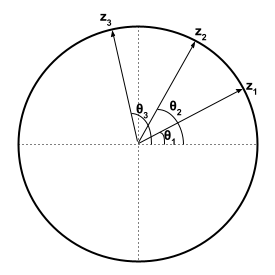
\includegraphics[width=0.5\textwidth]{figures/S1_Lie_group.png}
    \caption{S$_1$ group as Lie group.}
\end{figure}

This preserves the continuity of symmetry, so S$^1$ is smooth. 
Also, due to definition of multiplication and inversion, both the group operation of multiplication and inversion are also manifold.
This makes the group S$^1$ a Lie group. Moreover, the group operations are commutative, so the Lie group is \textbf{Abelian}.

\subsubsection{Lie Algebra}
An algebra, A over a field is a vector space over $\mathbb{C}$ equipped with bilinear product * defined as *:A $\times$ A $\rightarrow$ A.
Algebra is defined over a field implies that the vector space is also equipped with addition, multiplication, and scalar multiplication from the field.
Typically, algebra follows scalar multiplication and distributivity while commutativity and associativity are optional.
Let $\alpha, \beta, \gamma \: \epsilon$ A and c $\epsilon \: \mathbb{C}$ then

i. c ($\alpha * \beta$) = (c $\alpha) * \beta$ = $\alpha * (c \: \beta$) \\
ii. $\alpha * (\beta + \gamma $) = ($\alpha * \beta) + (\alpha* \gamma $)

Similarly, Lie algebra $\mathcal{L}$ is an algebra with operator [ , ] defined as [ , ]:$\mathcal{L} \times \mathcal{L} \rightarrow \mathcal{L}$.
Besides general properties of an algebra, Lie algebra has two other properties:
$\forall \: \alpha, \beta, \gamma \: \epsilon \: \mathcal{L}$

i. \textbf{skew-symmetry: } [$\alpha, \beta$] = - [$\beta, \alpha$] and [$\alpha, \alpha$] = 0 \\
ii. \textbf{Jacobi identity: } [$\alpha$, [$\beta, \gamma$]] + [$\beta$, [$\gamma, \alpha$]] + [$\gamma$, [$\alpha, \beta$]] = 0

These two properties are similar to vector multiplication.

\subsubsection{Exponential Map}
\href{https://en.wikipedia.org/wiki/Exponential_map_(Lie_theory)}{Exponential map} is a map from Lie algebra $\mathcal{L}$ of a Lie group \textbf{L} to the group, \textbf{exp:} $\mathcal{L} \rightarrow$ \textbf{L}, 
which allows one to recapture the local group structure from the Lie algebra. The ordinary exponential function is a special case of the exponential map when 
group G is the multiplicative group of positive real numbers (whose Lie algebra is the additive group of all real numbers).

The exponential of \textit{X} $\epsilon \: \mathcal{L}$ is denoted as \textbf{exp}(\textit{X}) and given by
\begin{equation}
    \textbf{exp}(X) = \sum_{k=0}^{\infty} \frac{X^k}{k!}
\end{equation}

If \textbf{L} be a \href{https://en.wikipedia.org/wiki/Lie_group#Matrix_Lie_groups}{matrix Lie group} then \textit{X} must have and inverse and det(\textit{X}) $\neq$ 0, so
there exists a matrix $\alpha$, logarithm of \textit{X} s.t.
\begin{equation}
    X = \textbf{exp}(\alpha) = \sum_{k=0}^{\infty} \frac{\alpha^k}{k!}
\end{equation}

The set of all matrices $\alpha$ whose exponentials belong to a group \textbf{L} is known as the Lie algebra, $\mathcal{L}$ of \textbf{L}.
Using the definition of the exponential series, we have
\begin{equation}
    X = \lim_{k \rightarrow \infty} \Big(I + \frac{\alpha}{k} \Big)^k \; \text{  and  } \; \alpha = \lim_{k \rightarrow \infty} k(X^{1/k}-I)
\end{equation}

For large k, the matrix (I + $\alpha$/k) is an operator of the group and gives \textit{X} by iteration. 
It is an \textbf{infinitesimal operator}, since for large k it differs from the identity operator by an infinitesimal amount.
Lie group is a manifold with a group structure and Lie algebra is its \textbf{tangent space}.
Elements of Lie algebra to a Lie group are sometimes referred to as \textbf{generators} of the group.
The Lie algebra can be thought of as the \textbf{infinitesimal vectors/operators} generating the group (at least locally) by means of
exponential map, but the Lie algebra doesn't form a generating set in strict sense.

\newpage

\section{PARTICLE PHYSICS}
\subsection{Discrete Symmetries}

\href{https://physics.stackexchange.com/questions/178986/how-is-jpc-value-experimentally-determined-for-new-types-of-particles}{\textbf{J}$^{\textbf{PC}}$}

\subsection{Spatial Rotations}
\textbf{Clebsch-Gordan coefficients}
\href{URL}{generator of rotations}
\href{https://en.wikipedia.org/wiki/Wigner_D-matrix}{Wigner D-matrix}

Helicity conservation in $e^+ e^- \rightarrow \mu^+ \mu^-$

Helicity, $\sigma$. $\frac{p}{|p|}$, is the projection of the spin along the momentum direction.

\subsection{Lorentz Invariance}
Most high-energy physics requires energy scales E $>>$ m$_p$, so it
is essential that the requirements of special relativity be respected. In
practice, this means identifying suitable 4-vectors and Lorentz invariants. 
Although the position and direction of particles is important when
actually performing experiments, the results are most often derived from
knowledge of the energy and momentum of the interacting particles.

\subsection{Rapidity}
High-energy hadron-hadron interactions tend to produce final states
with limited transverse momentum with respect to the initial beam direction. 
In such circumstances, rapidity (y) and transverse mass (m$_T$) are convenient variables.
\begin{equation}
    y = \frac{1}{2} ln \Big(\frac{E+p_z}{E-p_z}\Big), \hspace{1cm} m_T = \sqrt{m^2 + p_T^2}
\end{equation}


\newpage

\end{document}
